% !TEX TS-program = pdflatex
% !TEX encoding = UTF-8 Unicode

\documentclass{beamer}
%\documentclass[handout]{beamer}

%\setbeamertemplate{background canvas}[vertical shading][bottom=white,top=structure.fg!25]
% or whatever

\usetheme[compress]{Amsterdam}
%\setbeamertemplate{headline}{}
%\setbeamertemplate{footline}{}
%\setbeamersize{text margin left=0.5cm}
  
\usepackage[english]{babel}
\usepackage{listings}
\usepackage{geometry}
\usepackage{hyperref}

\usepackage{color}
\usepackage[T1]{fontenc}
\usepackage[utf8]{inputenc}
\usepackage{lmodern}
\usepackage{etoolbox}

\usepackage{tikz}
\usetikzlibrary{shapes,arrows}

\usepackage{multicol}
\lstset{
basicstyle=\scriptsize\ttfamily,
columns=flexible,
breaklines=true,
numbers=left,
%stepsize=1,
numberstyle=\tiny,
backgroundcolor=\color[rgb]{0.85,0.90,1}
}


\begin{document}

\title[Big Data and Automated Content Analysis]{\textbf{A Practical Introduction to Machine Learning in Python} \\Day 1 - Monday \\ »Introduction«}
\author[Damian Trilling, Anne Kroon]{Damian Trilling \\ Anne Kroon \\ ~ \\ \footnotesize{d.c.trilling@uva.nl, @damian0604 \\a.c.kroon@uva.nl, @annekroon} \\}
\date{March 9, 2020}
\institute[Gesis]{Gesis}


\tikzstyle{block} = [rectangle, draw, fill=blue!20, 
text width=5em, text centered, rounded corners, minimum height=4em]
\tikzstyle{line} = [draw]
\tikzstyle{pijltje} = [draw, -latex']
\tikzstyle{cloud} = [draw, ellipse,fill=red!20, node distance=3cm,
minimum height=2em, text width=4em, text centered,]



\begin{frame}{}
\titlepage
\end{frame}

\begin{frame}{Today}
\tableofcontents
\end{frame}

\section{Introducing\ldots}
\subsection{\ldots the people}

\begin{frame} 
Introducing\ldots \\
~~~~~~~~\ldots the people
\end{frame}


\begin{frame}{Introducing\ldots} {\huge{Damian}} \small{} 

\begin{columns}
	\column{.3\textwidth}
	\makebox[\columnwidth]{
		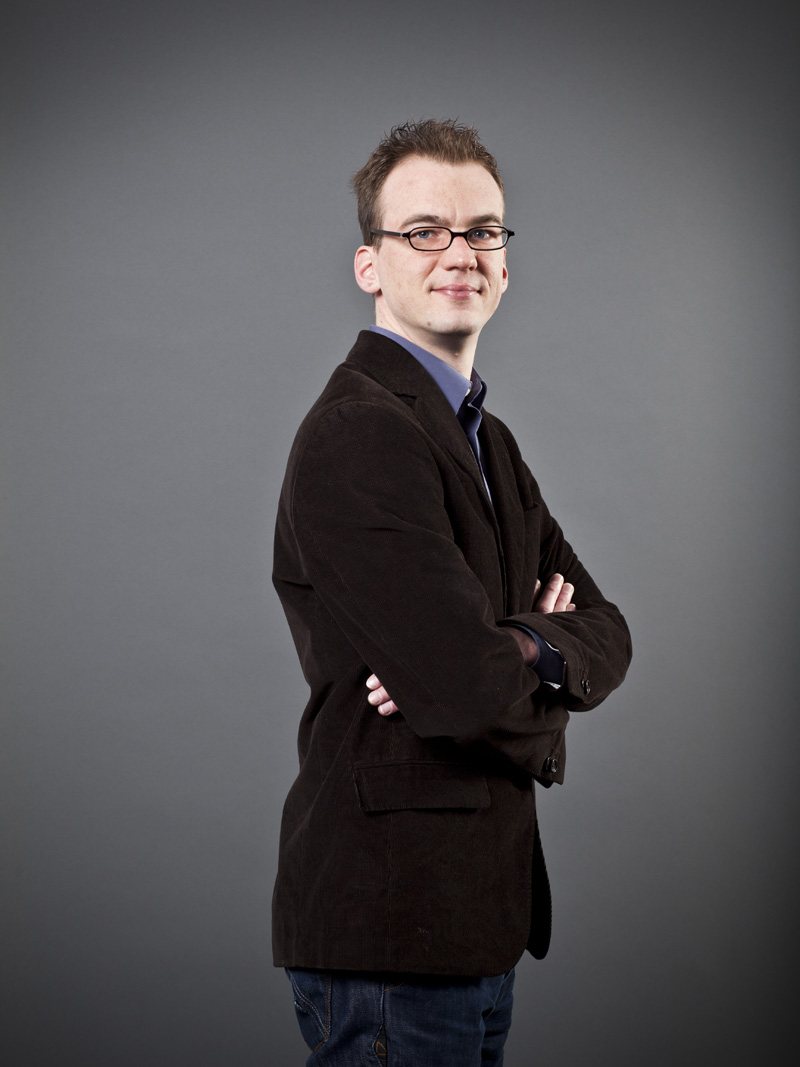
\includegraphics[width=\columnwidth,height=\paperheight,keepaspectratio]{../pictures/damian.jpg}}
	\column{.7\textwidth}
	dr. Damian Trilling \\
	Assistant Professor Political Communication \& Journalism \\
	\begin{itemize}
		%\item Studied Communication Science in M\"unster and at the VU 2003--2009
		%\item PhD candidate @ ASCoR 2009--2012
		\item interested in political communication and journalism in a changing media environment and in innovative (digital, large-scale, computational) research methods
	\end{itemize}
	@damian0604 \textbar d.c.trilling@uva.nl \textbar \url{www.damiantrilling.net} 
\end{columns}
\end{frame}

\begin{frame}{Introducing\ldots} {\huge{Anne}} \small{} 
\begin{columns}[] \column{.3\textwidth} \makebox[\columnwidth]{ 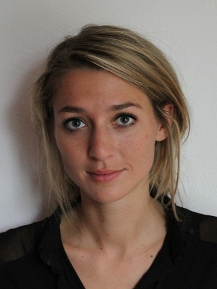
\includegraphics[width=\columnwidth,height=\paperheight,keepaspectratio]{../pictures/anne.jpg}} \column{.7\textwidth} dr. Anne Kroon \\ 
Assistant Professor Corporate Communication
\begin{itemize} 
	%\item Studied Journalism and Communication,  2006 - 2013
	%\item PhD candidate corporate communication at ASCoR (University of Amsterdam), 2014 - 2017
	\item Research focus on biased AI in recruitment, and media bias regarding minorities
	\item text analysis using automated approaches, word embeddings
\end{itemize} @annekroon \textbar a.c.kroon@uva.nl  \textbar \url{http://www.uva.nl/profiel/k/r/a.c.kroon/a.c.kroon.html} 
\end{columns} 
\end{frame}


\begin{frame}{Introducing\ldots}
{\huge{You}}
\small{}
\begin{columns}
\column{.3\textwidth}
\makebox[\columnwidth]{

\includegraphics[width=\columnwidth,height=\paperheight,keepaspectratio]{../pictures/mannetje.png}}
\column{.7\textwidth}
Your name?\\
Your background?\\
Your reason to follow this course?\\
Do you have a dataset you are working on?
\end{columns}
\end{frame}

\begin{frame}{Short poll}

Do you need
\begin{enumerate}[a]
	\item an intro
	\item a brief refresher
	\item nothing
\end{enumerate}

on

\begin{enumerate}[i]
	\item datatypes (int, float, string, lists, dictionaries)
	\item control flow statements (for, if, try/except)
	\item ways to run your code (notebooks vs IDE's vs text editors)
\end{enumerate}
?

\emph{We will try do adapt today's programme to your needs!}

\end{frame}


\section{Defining CSS}
\subsection{...some definitions}

\begin{frame}
What is Big Data?
\end{frame}

{\setbeamercolor{background canvas}{bg=black}
\begin{frame}[plain]
\makebox[\linewidth]{

\includegraphics[width=\paperwidth,height=\paperheight,keepaspectratio]{../pictures/teenage_sex}
}
\end{frame}
}

{\setbeamercolor{background canvas}{bg=black}
	\begin{frame}[plain]
	\makebox[\linewidth]{
		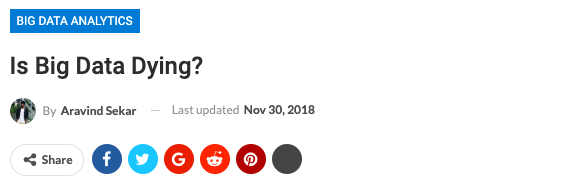
\includegraphics[width=\paperwidth,height=\paperheight,keepaspectratio]{../pictures/bigdata_dead}
	}
\end{frame}
}
%\begin{frame}{What is Big Data?}
%What would \emph{you} call Big Data?
%\end{frame}

\begin{frame}{What is Big Data?}
\begin{block}{A simple technical definition could be:}<2->
Everything that needs so much computational power and/or storage that you cannot do it on a regular computer.
\end{block}
\end{frame}

\begin{frame}{What is Big Data?}
\begin{block}{Vis, 2013}<2->
\begin{itemize}
\item<2,4> ``commercial'' definition (Gartner): ``'Big data' is high-volume, -velocity and -variety information assets that demand cost-effective, innovative forms of information processing for enhanced insight and decision making''
\item<3-> boyd \& Crawford definition: 
\begin{enumerate}
\item Technology: maximizing computation power and algorithmic accuracy to gather, analyze, link, and compare large data sets.
\item Analysis: drawing on large data sets to identify patterns in order to make economic, social, technical, and legal claims.
\item Mythology: the widespread belief that large data sets offer a higher form of intelligence and knowledge that can generate insights that were previously impossible, with the aura of truth, objectivity, and accuracy.
\end{enumerate}
\end{itemize}
\end{block}
\end{frame}


\begin{frame}{Implications \& criticism}
\begin{block}{boyd \& Crawford, 2012}<2->
\begin{enumerate}
\item Big Data changes the definition of knowledge
\item Claims to objectivity and accuracy are misleading
\item Bigger data are not always better data
\item Taken out of context, Big Data loses its meaning
\item Just because it is accessible does not make it ethical
\item Limited access to Big Data creates new digital divides
\end{enumerate}
\end{block}
\end{frame}


\begin{frame}{APIs, researchers and tools \emph{make} Big Data}
\begin{block}{Vis, 2013}<2->
Inevitable influences of:
\begin{itemize}
\item APIs
\item filtering, search strings, \ldots
\item changing services over time
\item organizations that provide the data
\end{itemize}
\end{block}
\end{frame}
% vraag stellen: maar is dit anders dan met andere soorten onderzoek? Of is dit een principieel (wetenschapsfilosofisch?) probleem?


\begin{frame}{Epistemologies and paradigm shifts}
\begin{block}{Kitchin, 2014}<1->
\begin{itemize}
\item<2-> (Reborn) empiricism: purely inductive, correlation is enough
\item<3-> Data-driven science: knowledge discovery guided by theory
\item<4-> Computational social science and digital humanities: employ Big Data research within existing epistemologies
\begin{itemize}
\item DH: descriptive statistics, visualizations
\item CSS: prediction and simulation
\end{itemize}
\end{itemize}
\end{block}
\end{frame}
% vraag stellen: maar is dit anders dan met andere soorten onderzoek? Of is dit een principiee

\subsection{Are we doing Big Data research?}

\begin{frame}{Are we doing Big Data research in this course?}
\begin{block}{Depends on the definition}<2->
\begin{itemize}
\item Not if we take a definition that \emph{only} focuses on computing power and the amount of data
\item<3-> \textbf{But:} We are using the same techniques. And they \emph{scale} well.
\item<4-> Oh, and about that high-performance computing in the cloud: We actually \emph{do} have access to that, so if someone has a really great idea\ldots
\end{itemize}

\end{block}
\end{frame}

\subsection{Computational social science}
\begin{frame}{Our epistomological underpinnings}
Computational Social Science
\end{frame}

\begin{frame}{Computational Social Science}
``It is an approach to social inquiry defined by (1) the use of large, complex datasets, often—though not always— measured in terabytes or petabytes; (2) the frequent involvement of “naturally occurring” social and digital media sources and other electronic databases; (3) the use of computational or algorithmic solutions to generate patterns and inferences from these data; and (4) the applicability to social theory in a variety of domains from the study of mass opinion to public health, from examinations of political events to social movements''

\vskip 0.5 cm
\tiny{Shah, D. V., Cappella, J. N., \& Neuman, W. R. (2015). Big Data, digital media, and computational social science: Possibilities and perils. T\textit{he ANNALS of the American Academy of Political and Social Science, 659}(1), 6–13. doi:10.1177/0002716215572084}
\end{frame}


\begin{frame}{Computational Social Science}
``[\ldots] the computational social sciences employ the scientific method, complementing descriptive statistics with inferential statistics that seek to identify associations and causality. In other words, they are underpinned by an epistemology wherein the aim is to produce sophisticated statistical models that explain, simulate and predict human life.''

\vskip 0.5 cm
\tiny{Kitchin, R. (2014). Big Data, new epistemologies and paradigm shifts. \textit{Big Data \& Society, 1}(1), 1–12. doi:10.1177/2053951714528481}
\end{frame}


\section{CSS project workflow}
\subsection{step-by-step}
\begin{frame}{Steps of a CSS project}
Different techniques for:
\begin{itemize}
	\item retrieving data (previous week)
	\item processing data (previous week)
	\item analyzing data (main part of this week)
	\item visualising data (a bit on Friday)
\end{itemize}

\end{frame}

\begin{frame}[plain]
\begin{tikzpicture}[node distance = 3cm, auto]
\node [cloud] (retrieve) {retrieve};
\node [cloud, right of=retrieve] (process) {process and/or enrich};
\node [cloud, right of=process] (analyze) {analyze\\ explain\\ predict};
\node [cloud, right of=analyze] (visualize) {communi-cate};


\path [pijltje] (retrieve)--(process);
\path [pijltje] (process)--(analyze);
\path [pijltje] (analyze)--(visualize);


\node [block, below of = retrieve] (retrievetech) {files\\ APIs\\ scraping};
\node [block, below of= process] (processtech) {NLP\\ sentiment\\ LDA\\ SML};
\node [block, below of=analyze] (analyzetech) {group comparisons; statistical tests and models};
\node [block, below of=visualize] (visualizetech) {visualizations and summary tables};


\path [pijltje] (retrievetech)--(processtech);
\path [pijltje] (processtech)--(analyzetech);
\path [pijltje] (analyzetech)--(visualizetech);


\node [block, below of = retrievetech, fill=green!20] (retrievepython) {glob\\ json \& csv\\ requests\\ lxml\\ \ldots};

\node [block, below of = processtech, fill=green!20] (processpython) {nltk\\ pattern \\ vader \\ gensim\\ scikit-learn \ldots};

\node [block, below of = analyzetech, fill=green!20] (analyzepython) {numpy/scipy\\ pandas\\ statsmodels\\ \ldots};

\node [block, below of = visualizetech, fill=green!20] (visualizepython) {pandas\\ matplotlib\\ seaborn\\ pyldavis\\ \ldots};

\path [line, dashed] (retrieve)--(retrievetech);
\path [line, dashed] (process)--(processtech);
\path [line, dashed] (analyze)--(analyzetech);
\path [line, dashed] (visualize)--(visualizetech);

\path [line, dashed] (retrievetech)--(retrievepython);
\path [line, dashed] (processtech)--(processpython);
\path [line, dashed] (analyzetech)--(analyzepython);
\path [line, dashed] (visualizetech)--(visualizepython);
\end{tikzpicture}
\end{frame}

\subsection{A good workflow}
\begin{frame}
	A good workflow
\end{frame}

\begin{frame}{The big picture}
\begin{block}{Start with pen and paper}
\begin{enumerate}[<+->]
	\item Draw the Big Picture
	\item Then work out what components you need
\end{enumerate}
\end{block}
\end{frame}

\section{Best practices}
\subsection{Open science}
\begin{frame}{Maximize transparency}
\begin{block}{Maximizing transparency of code and data}
	\begin{itemize}[<+->]
		\item Use openly accessible repository (e.g., Github)
		\item Store and preserve (pseudonymised) data at a secure environment (e.g., OSF)
		\item Create reusable workflows 
	\end{itemize}
\end{block}
\pause
\begin{exampleblock}{Advantages}
	\begin{itemize}[<+->]
		\item Reusable data and code
		\item Efficiency and credibility 
		\item Recognition of tools and data
	\end{itemize}
\end{exampleblock}

\end{frame}	

\subsection{Clean, high-quality code}
\begin{frame}{Develop components separately}
	\begin{block}{One script for downloading the data, one script for analyzing}
		\begin{itemize}[<+->]
			\item Avoids waste of resources (e.g., unnecessary downloading multiple times)
			\item Makes it easier to re-use your code or apply it to other data
		\end{itemize}
	\end{block}
\pause
\begin{block}{Start small, then scale up}
	\begin{itemize}[<+->]
		\item Take your plan and solve \textit{one} problem at a time (e.g., parsing a review page; or getting the URLs of all review pages)
		\item (for instance, by using functions [next slides])
	\end{itemize}
\end{block}

\end{frame}	

\begin{frame}{Develop components separately}
	\begin{block}{If you copy-paste code, you are doing something wrong}
		\begin{itemize}[<+->]
			\item Write loops!
			\item If something takes more than a couple of lines, write a function!
		\end{itemize}
	\end{block}
\end{frame}

\begin{frame}[plain, fragile]
Copy-paste approach\\ (ugly, error-prone, hard to scale up)
\begin{lstlisting}
allreviews = []

response = requests.get(`http://xxxxx')
tree =  fromstring(response.text)
reviewelements = tree.xpath(`//div[@class="review"]')
reviews = [e.text for e in reviewelements]
allreviews.extend(reviews)

response = requests.get(`http://yyyyy')
tree =  fromstring(response.text)
reviewelements = tree.xpath(`//div[@class="review"]')
reviews = [e.text for e in reviewelements]
allreviews.extend(reviews)
\end{lstlisting}
\end{frame}


\begin{frame}[plain, fragile]
Better: for-loop\\ (easier to read, less error-prone, easier to scale up (e.g., more URLs, read URLs from a file or existing list)
\begin{lstlisting}
allreviews = []

urls = [`http://xxxxx', `http://yyyyy']

for url in urls:
    response = requests.get(url)
    tree =  fromstring(response.text)
    reviewelements = tree.xpath(`//div[@class="review"]')
    reviews = [e.text for e in reviewelements]
    allreviews.extend(reviews)
\end{lstlisting}
\end{frame}


\begin{frame}[plain, fragile]
Even better: for-loop with functions\\ (main loop is easier to read, function can be re-used in multiple contexts)
\begin{lstlisting}
def getreviews(url):
    response = requests.get(url)
    tree =  fromstring(response.text)
    reviewelements = tree.xpath(`//div[@class="review"]')
    return [e.text for e in reviewelements]


urls = [`http://xxxxx', `http://yyyyy']

allreviews = []

for url in urls:
    allreviews.extend(getreviews(url))
\end{lstlisting}
\end{frame}

\subsection{datatypes}
\begin{frame}{Datatypes}
\begin{block}{Low-level: Native python datatypes}
	\begin{itemize}[<+->]
		\item Booleans, integers, floats, strings, bytes, byte arrays
		\item Lists, typles, sets, dictionaries
	\end{itemize}
\end{block}
\pause
\begin{exampleblock}{Advantages }
	\begin{itemize}[<+->]
		\item fast, flexible
		\item allows for nested, unstructured data 
	\end{itemize}
\end{exampleblock}
\pause
\begin{alertblock}{Disadvantages }
	\begin{itemize}[<+->]
		\item can be more cumbersome: e.g., inserting a column
		\item less consistency checks
	\end{itemize}
\end{alertblock}
\end{frame}


\begin{frame}{Datatypes}
\begin{block}{Higher-level: importing modules}
	\begin{itemize}[<+->]
		\item e.g., numpy, pandas, seaborn 
	\end{itemize}
\end{block}
\pause
\begin{exampleblock}{Advantages}
	\begin{itemize}[<+->]
		\item useful convenience functionality, works very intuitively (for tabular data)
		\item easy, allows for pretty visualization
	\end{itemize}
\end{exampleblock}
\pause
\begin{alertblock}{Disadvantages }
	\begin{itemize}[<+->]
		\item not suited for one-dimensional or messy / deeply nested data
		\item when your data is very large (machine learning!!)
	\end{itemize}
\end{alertblock}
\end{frame}

\begin{frame}{Datatypes in this course}
In this week, we will mainly work with lower-level datatypes (as opposed to, for instance, pandas dataframes)
\begin{itemize}[<+->]
	\item Often, ML algorithms require native data types as input (i.e., lists, genertors)
	\item We have to seriously consider memory:
	\item Maybe size does not apply to your project yet, but in the future you might want to scale up. 
\end{itemize}	
\end{frame}

\subsection{Generators}
\begin{frame}{Generators}
\begin{block}{Generators}
	\begin{itemize}[<+->]
		\item We will work with \textit{generators} to deal with memory issues
		\item Generators behave like iterators: loops through elements of an object. 
	\end{itemize}
\end{block}
\pause
\begin{exampleblock}{Behavior of a generator}
	\begin{itemize}[<+->]
		\item Does not hold results in memory
		\item Only computes results at the moment you need them (i.e. lazy')
		\item You can only loop over your object ONCE.
	\end{itemize}
\end{exampleblock}
\end{frame}

\begin{frame}[plain, fragile]
Creating generators: Example 1 
\begin{lstlisting}
def my_generator(my_list):	
    for i in my_list:
        yield i
example_list = [1, 2, 3, 4]
gen1 = my_generator(example_list)        
next(gen1)
\end{lstlisting}
\end{frame}


\begin{frame}[plain, fragile]
Creating generators: Example 2 (shorter)
\begin{lstlisting}
my_list = [1,2,3,4]
gen = (i for i in my_list)
\end{lstlisting}
\end{frame}


\subsection{Scaling up}
\begin{frame}{Scaling up}
When considering datatypes, consider re-usability, scalability
	\begin{itemize}
		\item Use functions and classes to make code more readable and re-usable
		\item Avoid re-calculating values
		\item Think about how to minimize memory usage (e.g., Generators)
		\item Do not hard-code values, file names, etc., but take them as arguments
	\end{itemize}	
\end{frame}


\begin{frame}{Make it robust}
You cannot foresee every possible problem.\\
Most important: Make sure your program does not fail and loose all data just because something goes wrong at case 997/1000.
	\begin{itemize}
		\item Use \texttt{try/except} to explicitly tell the program how to handle errors
		\item Write data to files (or database) in between
		\item Use \texttt{assert len(x) == len(y}) for sanity checks
	\end{itemize}	
\end{frame}

\subsection{data storage}
\begin{frame}{Storing data}
\begin{block}{Use of databases}
	Storing data
	\begin{itemize}
		\item We can store our data in files (often, one CSV or JSON file)
		\item But that's not very efficient if we have large datasets; especially if we want to select subsets later on
		\item SQL-databases to store tables (e.g., MySQL)
		\item NoSQL-databases to store less structured data (e.g., JSON with unknown keys) (e.g., MongoDB, ElasticSearch)
		\item $\Rightarrow$ \tiny{Günther, E., Trilling, D., \& Van de Velde, R.N. (2018). But how do we store it? (Big) data architecture in the social-scientific research process. In:\textit{ Stuetzer, C.M., Welker, M., \& Egger, M. (eds.): Computational Social Science in the Age of Big Data. Concepts, Methodologies, Tools, and Applications}. Cologne, Germany: Herbert von Halem.}
	\end{itemize}
\end{block}
\end{frame}

\begin{frame}{Storing data}
\makebox[\linewidth]{
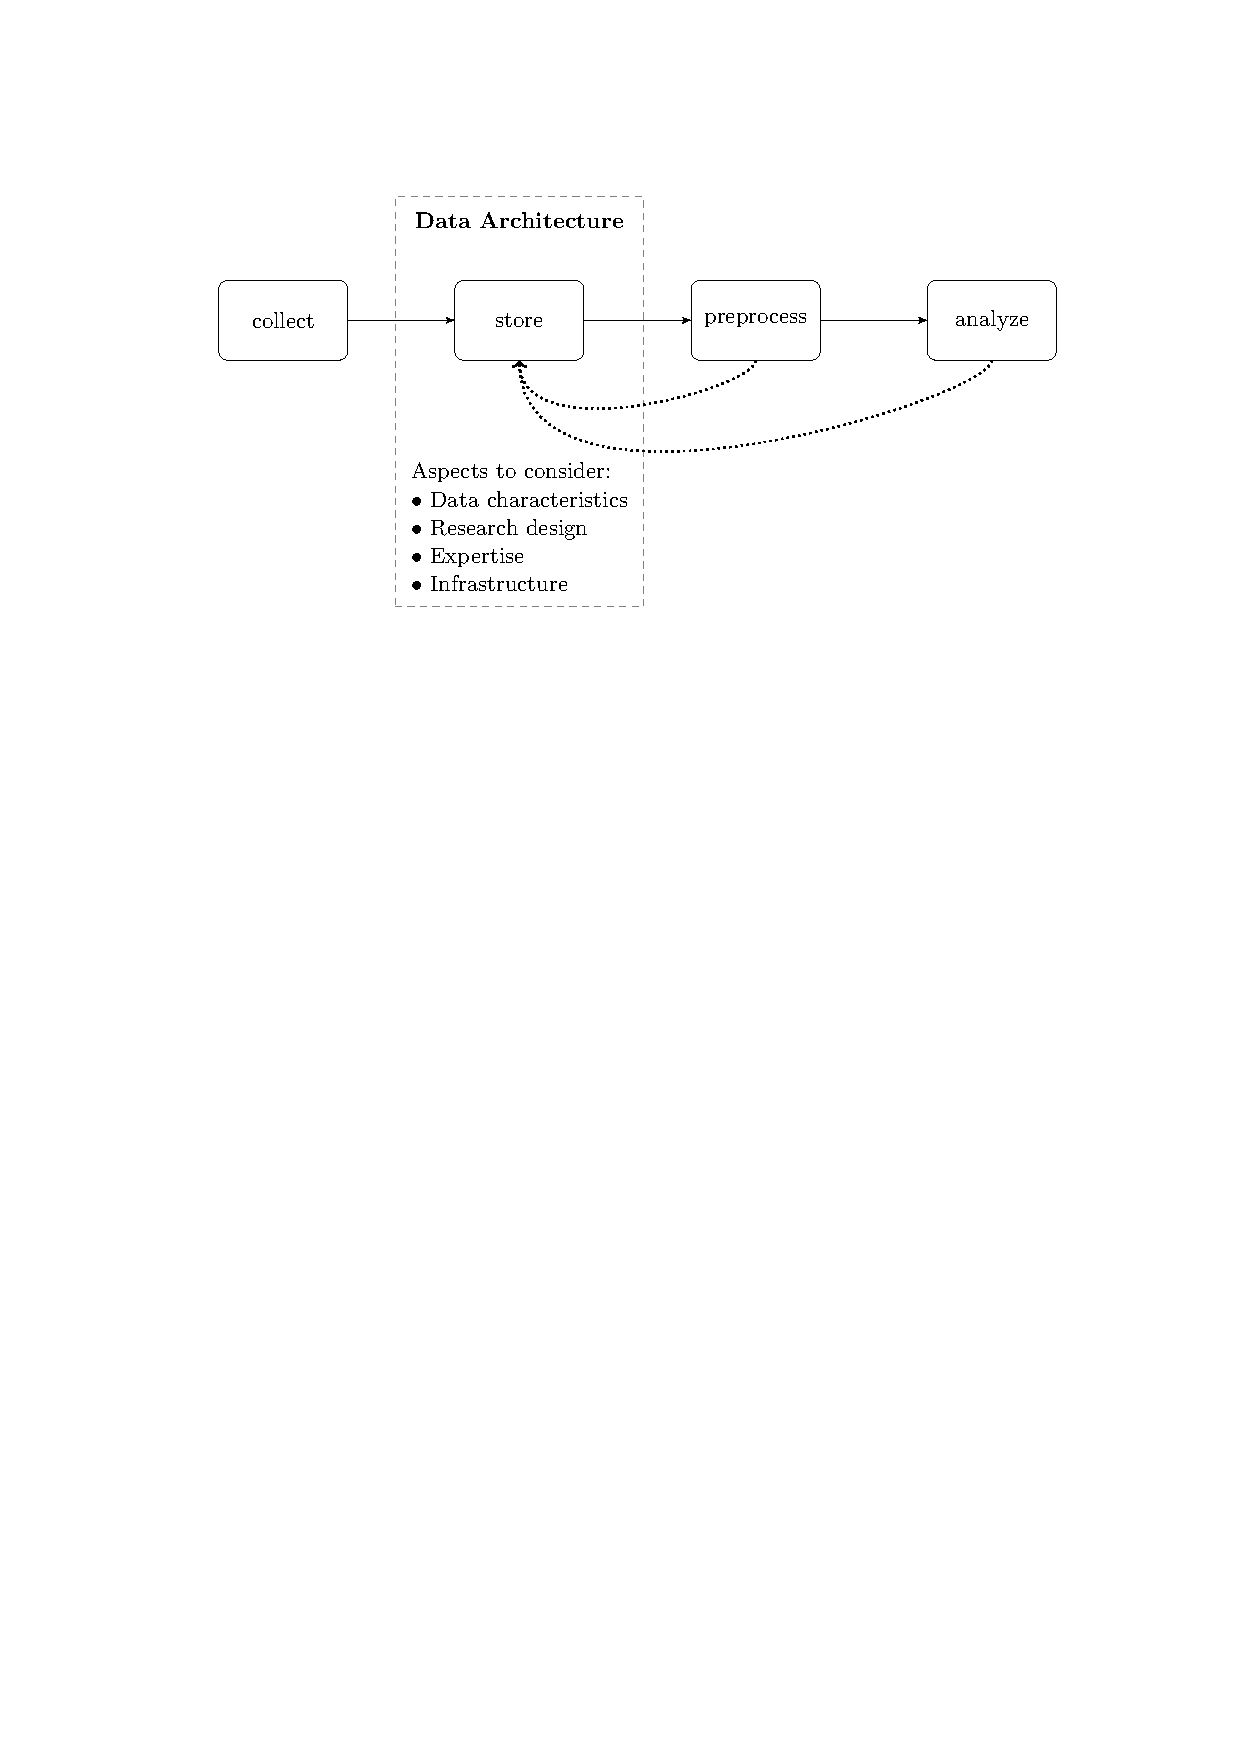
\includegraphics[width=\paperwidth,height=\paperheight,keepaspectratio]{../pictures/guenteretal_fig1}}
\end{frame}

\begin{frame}{From retrieved data to enriched data}
\makebox[\linewidth]{
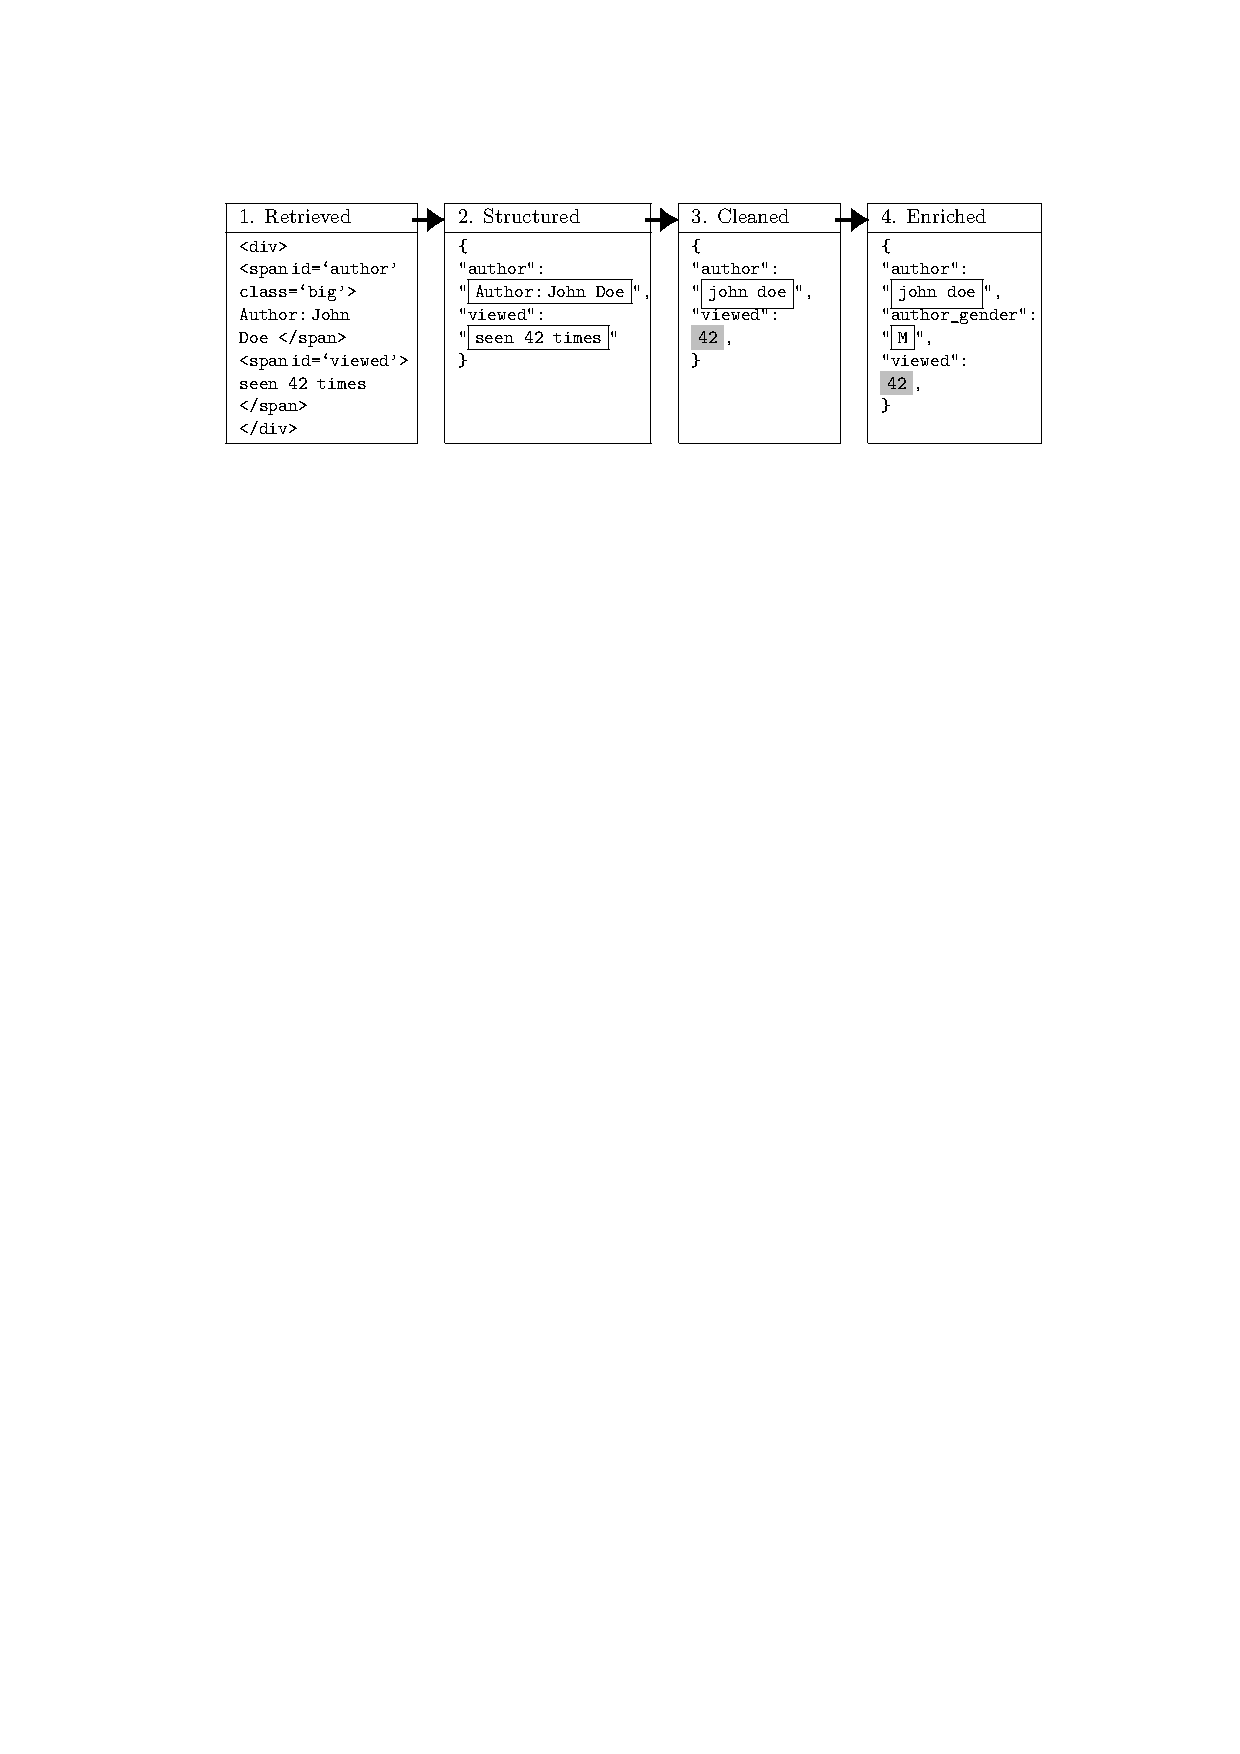
\includegraphics[width=\paperwidth,height=\paperheight,keepaspectratio]{../pictures/guentheretal_fig3}}
\end{frame}


\section{Looking forward}
\subsection{And now you... }
\begin{frame}[plain]{}
Looking forward\\
\textbf{Try to fill in the blanks for your personal CSS project}
\end{frame}


\begin{frame}[plain]
	\begin{tikzpicture}[node distance = 3cm, auto]
	\node [cloud] (retrieve) {retrieve};
	\node [cloud, right of=retrieve] (process) {process and/or enrich};
	\node [cloud, right of=process] (analyze) {analyze\\ explain\\ predict};
	\node [cloud, right of=analyze] (visualize) {communi-cate};
	
	
	\path [pijltje] (retrieve)--(process);
	\path [pijltje] (process)--(analyze);
	\path [pijltje] (analyze)--(visualize);
	
	
	\node [block, below of = retrieve] (retrievetech) {?};
	\node [block, below of= process] (processtech) {?};
	\node [block, below of=analyze] (analyzetech) {?};
	\node [block, below of=visualize] (visualizetech) {?};
	
	
	
	\path [pijltje] (retrievetech)--(processtech);
	\path [pijltje] (processtech)--(analyzetech);
	\path [pijltje] (analyzetech)--(visualizetech);
	
	
	\node [block, below of = retrievetech, fill=green!20] (retrievepython) {?};
	
	\node [block, below of = processtech, fill=green!20] (processpython) {?};
	
	\node [block, below of = analyzetech, fill=green!20] (analyzepython) {?};
	
	\node [block, below of = visualizetech, fill=green!20] (visualizepython) {?};
	
	
	
	
	
	\path [line, dashed] (retrieve)--(retrievetech);
	\path [line, dashed] (process)--(processtech);
	\path [line, dashed] (analyze)--(analyzetech);
	\path [line, dashed] (visualize)--(visualizetech);
	
	
	
	\path [line, dashed] (retrievetech)--(retrievepython);
	\path [line, dashed] (processtech)--(processpython);
	\path [line, dashed] (analyzetech)--(analyzepython);
	\path [line, dashed] (visualizetech)--(visualizepython);
	\end{tikzpicture}
\end{frame}



\begin{frame}[plain]
Long story short:

\textbf{Don't forget to plan the bigger picture}

We will focus on machine learning this week. But for each technique we cover, think about how it fits in \emph{your} workflow.

\pause

\ldots and now lets get started!

\end{frame}

\section[The ACA toolkit]{The Automated Content Analysis toolkit}
\begin{frame}{}
Types of Automated Content Analysis
\end{frame}

\subsection*{Top-down vs. bottom-up}

%{\setbeamercolor{background canvas}{bg=black}
\begin{frame}[plain]
\makebox[\linewidth]{
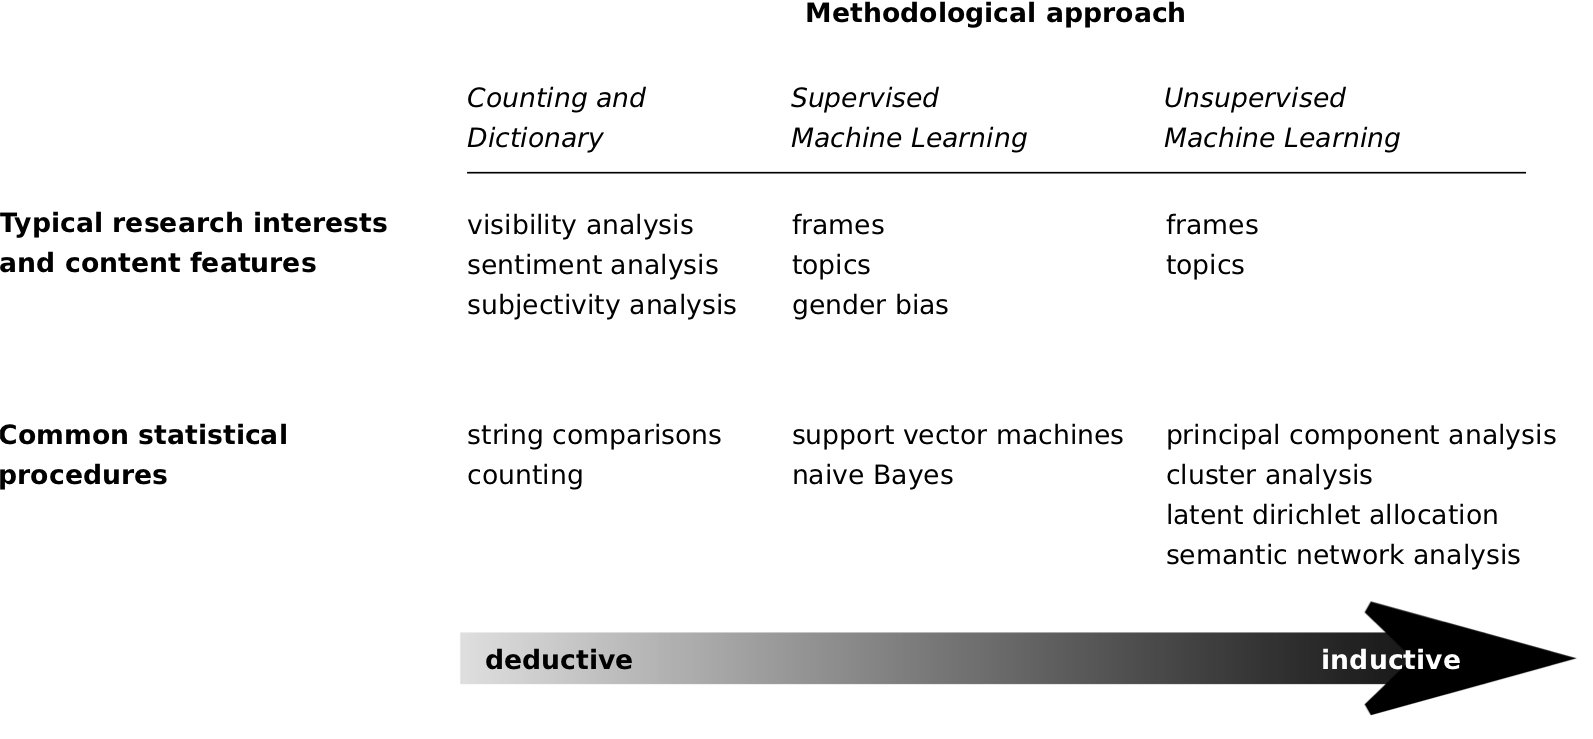
\includegraphics[width=\paperwidth,height=\paperheight,keepaspectratio]{../pictures//boumanstrilling2016_.png}}
\end{frame}
%}

\begin{frame}{Some terminology }
\begin{columns}[t]
\column{.5\textwidth}

\begin{block}<1-4>{Supervised machine learning}
You have a dataset with both predictor and outcome (independent and dependent variables; features and labels) --- a \emph{labeled} dataset.
\onslide<2>{
	\footnotesize{Think of regression: You measured \texttt{x1}, \texttt{x2}, \texttt{x3} and you want to predict \texttt{y}, which you also measured}}
\end{block}

\column{.5\textwidth}

\begin{block}<3->{Unsupervised machine learning}
You have no labels. \onslide<4>{(\footnotesize{You did not measure \texttt{y})}}\\
\onslide<5>{\textbf{Again, you already know some techniques to find out how \texttt{x1}, \texttt{x2},\ldots \texttt{x\_i} co-occur from other courses:} \begin{itemize}
		\item Principal Component Analysis (PCA)
		\item Cluster analysis
		\item \ldots
	\end{itemize}
}
\end{block}

\end{columns}

\end{frame}


\section{Final}

\begin{frame}{This afternoon}
\begin{block}{Getting started}
	Getting started with the IMBD dataset
\end{block}
\end{frame}





\section{Backupslides basics}

\begin{frame}[plain]
\centering
\huge
Backup slides in case we need to do more fundamentals
\end{frame}



\section*[Basics]{The very, very, basics of programming with Python}
\begin{frame}[plain]
\textbf{The very, very, basics of programming}\\
\vspace{1cm}
See also Chapter 4.
\end{frame}
\subsection*{Datatypes}


\begin{frame}{Python lingo}
\begin{block}{Basic datatypes (variables)}
\begin{description}
\item[{\color{red}int}] \texttt{32}
\item[{\color{red}float}] \texttt{1.75}
\item[{\color{red}bool}] \texttt{True}, \texttt{False}
\item[{\color{red}string}] \texttt{"Damian"}
\onslide<2->{\scriptsize \item[({\color{red}variable name}] \texttt{firstname})}
\end{description}
\end{block}
\onslide<2->{\textbf{"firstname" and firstname is not the same.\\}}
\onslide<3->{\textbf{"5" and 5 is not the same.}\\ But you can transform it: {\tt{int("5")}} will return 5.}\\
\onslide<3->{\textbf{You cannot calculate \texttt{3 * "5"}} {\tiny{(In fact, you can. It's \tt{"555"})}}.\\
But you can calculate {\tt{3 * int("5")}}}
\end{frame}



\begin{frame}{Python lingo}
\begin{block}{More advanced datatypes}
\begin{description}
\item[{\color{red}list}]<2-> \texttt{firstnames = $[$'Damian','Lori','Bjoern'$]$ \\ lastnames = $[$'Trilling','Meester','Burscher'$]$}
\item[{\color{red}list}]<3->\texttt{ages = $[$18,22,45,23$]$}
\item[{\color{red}dict}]<4-> \texttt{familynames= \{'Bjoern': 'Burscher', 'Damian': 'Trilling', 'Lori': 'Meester'\} }
\item[{\color{red}dict}]<4-> \texttt{\{'Bjoern': 26, 'Damian': 31, 'Lori': 25\} }

\end{description}
\pause
Note that the elements of a list, the keys of a dict, and the values of a dict can have any datatype! (Better to be consistent, though!)
\end{block}
\end{frame}


\subsection*{Functions and methods}
\begin{frame}{Python lingo}
\begin{block}{Functions}
\begin{description}
\item[{\color{red}functions}]<2-> Take an input and return something else \\ {\tt{int(32.43})} returns the integer 32. \texttt{len("Hello")} returns the integer 5.\\ 
\item[{\color{red}methods}]<3-> are similar to functions, but directly associated with an object. {\tt{"SCREAM".lower()}} returns the string "scream"
\end{description}
\end{block}
\onslide<4->{Both functions and methods end with \texttt{()}. Between the \texttt{()}, \emph{arguments} can (sometimes have to) be supplied.}
\end{frame}


\begin{frame}[fragile]{Writing own functions}
You can write an own function:
\begin{lstlisting}
def addone(x):
    y = x + 1
    return y
\end{lstlisting}

Functions take some input (``argument'') (in this example, we called it \texttt{x}) and \emph{return} some result.
	
Thus, running
\begin{lstlisting}	
addone(5)
\end{lstlisting}
returns \tt{6}.
\end{frame}



\subsection*{Modifying lists and dictionaries}

\begin{frame}[plain]
Modifying lists and dictionaries
\end{frame}{}
	
\begin{frame}[fragile]{Modifying lists}
\begin{block}{Appending to a list}
\begin{lstlisting}
mijnlijst = ["element 1", "element 2"]
anotherone = "element 3"   # note that this is a string, not a list!
mijnlijst.append(anotherone)
print(mijnlijst)
\end{lstlisting}
gives you:
\begin{lstlisting}
["element 1", "element 2", "element 3"]
\end{lstlisting}
\end{block}
\end{frame}



\begin{frame}[fragile]{Modifying lists}
\begin{block}{Merging two lists (= extending)}
\begin{lstlisting}
mijnlijst = ["element 1", "element 2"]
anotherone = ["element 3", "element 4"]
mijnlist.extend(anotherone)
print(mijnlijst)
\end{lstlisting}
gives you:
\begin{lstlisting}
["element 1", "element 2", "element 3", "element 4]
\end{lstlisting}
\end{block}
\end{frame}




\begin{frame}[fragile]{Modifying dicts}
\begin{block}{Adding a key to a dict (or changing the value of an existing key)}
\begin{lstlisting}
mydict = {"whatever": 42, "something": 11}
mydict["somethingelse"] = 76
print(mydict)
\end{lstlisting}
gives you:
\begin{lstlisting}
{'whatever': 42, 'somethingelse': 76, 'something': 11}
\end{lstlisting}
If a key already exists, its value is simply replaced.
\end{block}
\end{frame}




\subsection*[Indention]{Indention: The Python way of structuring your program}
\begin{frame}[plain]
Indention: The Python way of structuring your program
\end{frame}


\begin{frame}[fragile]{Indention}
\begin{block}{Structure}
The program is structured by TABs or SPACEs
\end{block}

\end{frame}



{\setbeamercolor{background canvas}{bg=black}
\begin{frame}[plain]
\makebox[\linewidth]{
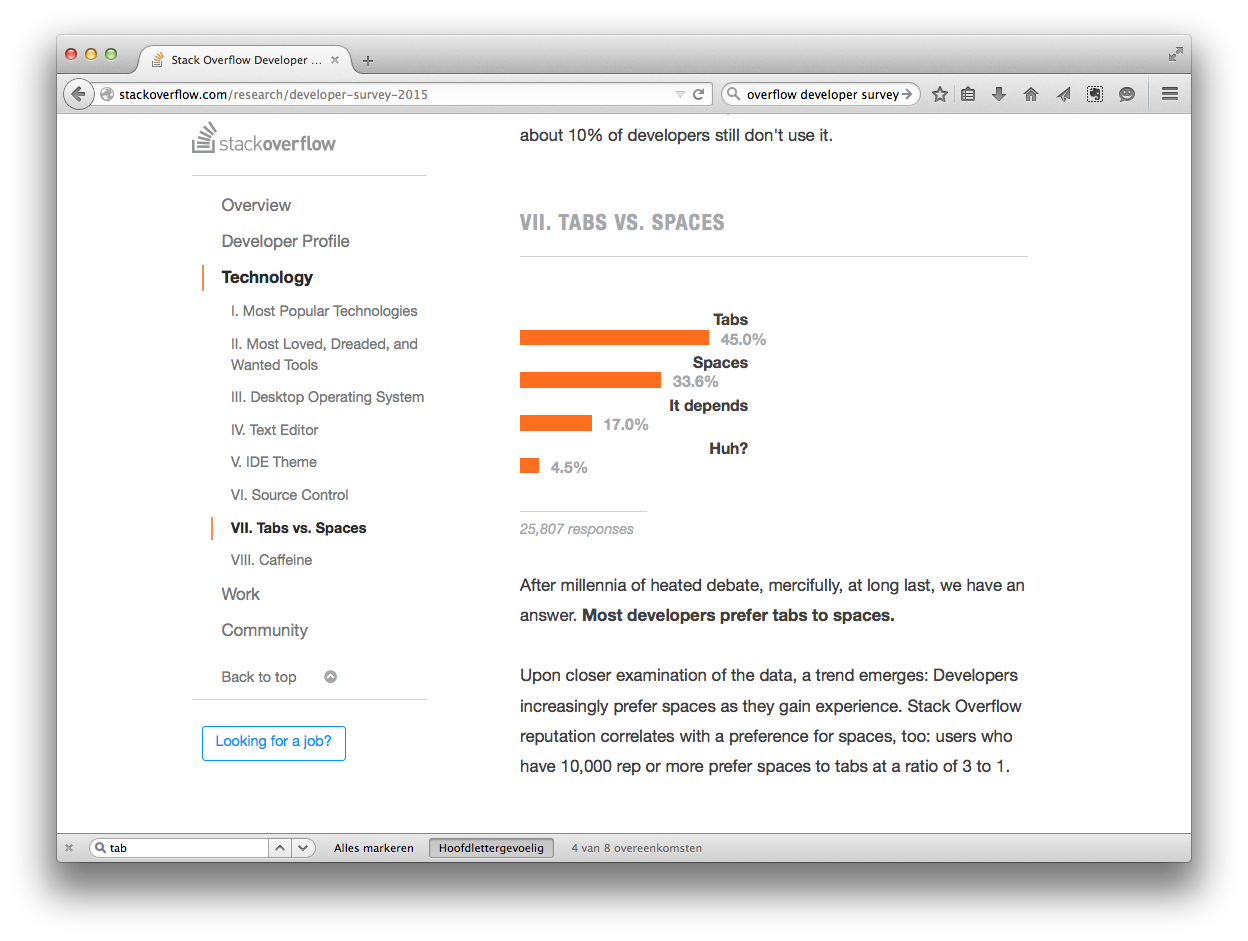
\includegraphics[width=\paperwidth,height=\paperheight,keepaspectratio]{../pictures/tabsvsspaces}
}
\end{frame}
}

\begin{frame}[fragile]{Indention}
\begin{block}{Structure}
The program is structured by TABs or SPACEs
\end{block}
\begin{lstlisting}
firstnames=['Damian','Lori','Bjoern']
age={'Bjoern': 27, 'Damian': 32, 'Lori': 26}
print ("The names and ages of these people:")
for naam in firstnames:
    print (naam,age[naam])
\end{lstlisting}
\onslide<2->{\textbf{Don't mix up TABs and spaces! Both are valid, but you have to be consequent!!! Best: always use 4 spaces!}}
\end{frame}





\begin{frame}[fragile]{Indention}
\begin{block}{Structure}
The program is structured by TABs or SPACEs
\end{block}
\begin{lstlisting}
print ("The names and ages of all these people:")
for naam in firstnames:
    print (naam,age[naam])
    if naam=="Damian":
        print ("He teaches this course")
    elif naam=="Lori":
        print ("She is a former assistant")
    elif naam=="Bjoern":
        print ("He helped teaching this course in the past")
    else:
        print ("No idea who this is")
\end{lstlisting}
\end{frame}


\begin{frame}{Indention}
The line \emph{before} an indented block starts with a \emph{statement} indicating what should be done with the block and ends with a \texttt{:}

\begin{block}{Indention of the block indicates that}<2->
\begin{itemize}
\item<3-> it is to be executed repeatedly (\texttt{for} statement) – e.g., for each element from a list
\item<4-> it is only to be executed under specific conditions (\texttt{if}, \texttt{elif}, and \texttt{else} statements)
\item<5-> an alternative block should be executed if an error occurs (\texttt{try} and \texttt{except} statements)
\item<6-> a file is opened, but should be closed again after the block has been executed (\texttt{with} statement)
\end{itemize}
\end{block}
\end{frame}


\section*{Exercise}
\subsection**{Exercise}
\begin{frame}
We'll now together do some simple exercises \ldots
\end{frame}



\begin{frame}{Exercises}
\begin{block}{1. Warming up}
\begin{itemize}
	\item Create a list, loop over the list, and do something with each value (you're free to choose). 
\end{itemize}
\end{block}
\begin{block}{2. Did you pass?}
	\begin{itemize}
	\item Think of a way to determine for a list of  grades whether they are a pass (>5.5) or fail.
	\item Can you make that program robust enough to handle invalid input (e.g., a grade as 'ewghjieh')?
	\item How does your program deal with impossible grades (e.g., 12 or -3)?
	\item \ldots
\end{itemize}
\end{block}
\end{frame}



\end{document}

